%% JSS Submission — Elsevier elsarticle template
%% Paper: "The Dynamics of Joy in Software Creation:
%%         Transparency, Flow, and Motivational Archetypes"
%% Authors: Alfonso Pierantonio, Bernhard Schenkenfelder
%%
%% Compiled with: pdflatex / xelatex
%% Required packages: elsarticle, standard LaTeX packages listed below

\documentclass[12pt]{elsarticle}

%% ---------------------------------------------------------------
%% PACKAGES
%% ---------------------------------------------------------------
\usepackage{lineno}          % line numbers for review
\usepackage{hyperref}        % clickable references
\usepackage{booktabs}        % professional tables
\usepackage{tabularx}        % flexible-width tables
\usepackage{multirow}        % multirow cells
\usepackage{graphicx}        % figures
\usepackage{amsmath}         % equations
\usepackage{amssymb}
\usepackage{xcolor}          % coloured text if needed
\usepackage{microtype}       % better typography
\usepackage{cleveref}        % smart cross-references

%% JSS uses numbered references (Vancouver style)
\bibliographystyle{elsarticle-num}

%% Enable line numbers during review
%\linenumbers

%% ---------------------------------------------------------------
%% JOURNAL METADATA
%% ---------------------------------------------------------------
\journal{Journal of Systems and Software}

%% ---------------------------------------------------------------
%% FRONT MATTER
%% ---------------------------------------------------------------
\begin{document}

\begin{frontmatter}

%% Title
\title{The Dynamics of Joy in Software Creation:\\
Transparency, Flow, and Motivational Archetypes}

%% Authors and affiliations
%% Use \fnref and \ead for footnotes / email
\author[univaq]{Alfonso Pierantonio\corref{cor1}}
\ead{alfonso.pierantonio@univaq.it}

\author[scch]{Bernhard Schenkenfelder}
\ead{bernhard.schenkenfelder@scch.at}

\cortext[cor1]{Corresponding author}

\affiliation[univaq]{
    organization={DISIM, Universit\`{a} degli Studi dell'Aquila},
    addressline={Via Vetoio, Coppito},
    city={L'Aquila},
    postcode={67100},
    country={Italy}
}

\affiliation[scch]{
    organization={Software Competence Center Hagenberg},
    city={Hagenberg},
    country={Austria}
}

%% ---------------------------------------------------------------
%% ABSTRACT
%% ---------------------------------------------------------------
\begin{abstract}
Understanding why software creation can be deeply joyful for some 
developers and not for others requires an integrated account of 
cognition, motivation, and tool experience. In this paper, we 
conceptualize joy as the experiential outcome of three interacting 
mechanisms: the transparency of tools and representations, the 
emergence of flow-like cognitive absorption, and an individual's 
underlying motivational orientation. Drawing on psychological 
theory, phenomenology, and research on software engineering 
cognition, we derive six motivational dimensions---Growth, 
Resolution, Coherence, Creation, Contribution, and Autonomy---that 
structure how developers interpret and value their work. Using these 
dimensions, we construct a theory-driven typology of twelve 
archetypes, each representing a distinct motivational profile that 
shapes the conditions under which joy emerges. We present a 
conceptual model that describes how contextual factors, friction, 
attentional dynamics, and motivational sensitivity jointly influence 
the experiential quality of software work. Together, the model and 
typology help explain why identical tools or workflows can generate 
profoundly different experiences between individuals. We conclude 
with implications for the design of developer tools, practices, and 
socio-technical environments that more effectively support 
meaningful, sustainable, and joyful software creation.
\end{abstract}

%% ---------------------------------------------------------------
%% HIGHLIGHTS  (Elsevier requirement: 3-5 items, max 85 chars each)
%% ---------------------------------------------------------------
\begin{highlights}
\item Joy in software creation emerges from transparency, flow, and motivational alignment.
\item Six motivational dimensions structure developers' experiential responses to software work.
\item A typology of twelve archetypes captures distinct motivational pathways toward joy.
\item Identical tools generate different experiences depending on motivational orientation.
\item Design implications target friction reduction, motivational diversity, and team composition.
\end{highlights}

%% ---------------------------------------------------------------
%% KEYWORDS
%% ---------------------------------------------------------------
\begin{keyword}
Developer Experience \sep
Flow and Engagement \sep
Tool Transparency \sep
Motivation and Reward \sep
Practitioner Typologies \sep
Software Engineering Cognition
\end{keyword}

\end{frontmatter}

%% ---------------------------------------------------------------
%% MAIN TEXT
%% ---------------------------------------------------------------

\section{Introduction}
\label{sec:introduction}

Joy is rarely treated as a first-class concept in software engineering 
or human--computer interaction, yet developers frequently describe 
moments of exhilaration, clarity, and meaningfulness during software 
creation. These episodes are not incidental; they arise when cognitive, 
motivational, and environmental conditions align in ways that support 
fluid interaction and sustained engagement. Understanding the nature of 
this joy of software creation is therefore essential for improving 
developer experience, well-being, and the quality of socio-technical 
environments~\cite{ford2015,graziotin2014}.

Research in psychology shows that intrinsic motivation emerges when 
individuals experience competence, autonomy, and meaningful 
challenge~\cite{deci2013,ryan2000}, and that positive affect broadens 
attention and supports creative problem solving~\cite{fredrickson2001}. 
Flow theory further explains how deep absorption in an activity arises 
when skills and challenges are well matched and when feedback is 
immediate and interpretable~\cite{csikszentmihalyi1990}. 
Phenomenological treatments of tool use show that transparency and felt 
immediacy are essential for seamless interaction~\cite{heidegger1962,ihde1990}. 
In software engineering, studies of developer cognition highlight the 
importance of stable mental models, predictable feedback, and 
uninterrupted focus~\cite{parnin2011,soloway2009}.

In this paper, we argue that joyful participation in software creation 
emerges from the interaction of three mechanisms: the transparency of 
tools and representations, flow-like absorption in the task, and 
individuals' underlying motivational orientation. Motivational 
orientation is shaped by four well-established psychological components: 
values, reward sensitivity, cognitive style, and reinforcement 
history~\cite{gray1987,messick1976}. These components jointly determine 
what kinds of activity feel meaningful or energizing to a practitioner. 
Building on these dimensions, we synthesize six motivational 
dimensions---Growth, Resolution, Coherence, Creation, Contribution, and 
Autonomy---that structure the experiential responses of developers to 
software work.

Although prior research has examined affect in programming, cognitive 
load, developer productivity, and flow states~\cite{csikszentmihalyi1990,
ford2015,graziotin2014,parnin2011}, existing studies rarely integrate 
these perspectives into a unified account of joyful engagement. Moreover, 
most work assumes relatively uniform motivational responses among 
developers, overlooking substantial individual differences in how and why 
joy arises. To address this gap, we develop a conceptual model of joyful 
software engagement and introduce a typology of twelve motivational 
archetypes derived through a systematic theory-driven synthesis.

\medskip
\noindent\textbf{Paper structure.}
\Cref{sec:background} reviews related work on affect, cognition, and 
phenomenology in software engineering. \Cref{sec:foundations} introduces 
the conceptual foundations of transparency, flow, and motivational 
orientation. \Cref{sec:methodology} describes the theory-driven 
methodology. \Cref{sec:deriving} details the archetype derivation 
process. \Cref{sec:archetypes} presents the twelve archetypes. 
\Cref{sec:model} introduces the experiential model. \Cref{sec:typology} 
analyzes cross-archetype relationships. \Cref{sec:design} discusses 
design implications. \Cref{sec:threats} addresses threats to validity, 
and \Cref{sec:conclusion} concludes.

% ---------------------------------------------------------------
\section{Background and Related Work}
\label{sec:background}

Research on human aspects of software engineering has expanded 
substantially in the past decade, with increasing attention to cognition, 
affect, and developer experience (DX). Previous work suggests that tool 
usability, workflow design, and socio-technical factors influence 
productivity, cognitive load, and emotional 
states~\cite{graziotin2017,graziotin2015}. Emotions such as frustration, 
confusion, satisfaction, and happiness correlate with development 
outcomes~\cite{muller2015}, yet affect is often examined only in terms 
of valence or its impact on productivity. The notion of joy as a 
structured experiential phenomenon, rather than a transient emotion, 
remains under-theorized.

Flow theory~\cite{csikszentmihalyi1990} provides one of the most 
influential accounts of deep engagement and has been widely referenced 
in software engineering. Prior studies indicate that uninterrupted 
attention, clear feedback, and a balanced relationship between challenge 
and skill contribute to entering and maintaining flow~\cite{ford2015}. 
However, existing work does not explain how flow becomes joyful or why 
different developers experience the emotional quality of flow in different 
ways. Our work addresses this gap by treating flow as a mechanism through 
which joy emerges, moderated by motivational differences.

The concept of transparency, rooted in phenomenology, further informs 
how tool design shapes experience. Heidegger's account of 
readiness-to-hand describes how tools disappear from conscious awareness 
when they function seamlessly during skilled 
activity~\cite{heidegger1962}, and Ihde's postphenomenological 
perspective emphasizes how technologies mediate and shape 
experience~\cite{ihde1990}. In HCI, transparency has been associated 
with the reduction of cognitive friction and smoother action 
possibilities~\cite{dourish2001}. Closely related is the rich body of 
work on cognitive load and distributed cognition~\cite{hutchins1995,
sweller1988}, which highlights how the mental cost of interacting with 
representations affects performance. Software engineering research also 
links transparency to abstraction and cognitive 
alignment~\cite{kramer2007}, suggesting that well-calibrated abstractions 
reduce overhead and facilitate reasoning about complex systems. Building 
on these foundations, we conceptualize transparency as a prerequisite 
for flow and, indirectly, for joy.

Understanding joy also requires psychological research on motivation, 
values, and individual differences. Self-Determination Theory identifies 
autonomy, competence, and relatedness as key psychological 
needs~\cite{ryan2000}, while values theory explains differences in what 
individuals find meaningful~\cite{schwartz1992}. Cognitive style research 
demonstrates that people differ in how they process information and 
approach problem solving~\cite{kozhevnikov2007}. Reinforcement learning 
perspectives further show how past experience shapes patterns of reward 
sensitivity and preferred modes of engagement~\cite{anderson2000}.

Together, these strands of research highlight the importance of affect, 
flow, cognitive load, and tool transparency in shaping developers' 
experiences. However, they also reveal a gap: existing work explains how 
engagement is supported or disrupted, but not why the same conditions 
produce different experiential outcomes across individuals. Addressing 
this gap requires a conceptual account that links cognitive mechanisms to 
stable motivational sensitivities.

% ---------------------------------------------------------------
\section{Theoretical Foundations}
\label{sec:foundations}

To explain why joyful engagement arises unevenly between practitioners, 
we build on three complementary theoretical constructs: the transparency 
of tools and representations, the emergence of flow-like cognitive 
absorption, and the motivational orientations that shape how individuals 
interpret and value their work.

\subsection{Joy as Frictionless Engagement}

We conceptualize joy as the affective quality that arises when cognitive 
processing unfolds with minimal friction. Joy is not just a positive 
emotion, but a structural property of a cognitive system that operates 
in a mode of alignment. When actions, representations, and intentions 
cohere without interruption, the individual experiences a state of 
\emph{cognitive smoothness}. This smoothness is intrinsically pleasurable 
because it signals predictive success, stable control, and the absence 
of cognitive conflict~\cite{berridge2012}. Joy is therefore an emergent 
property of a frictionless cognitive dynamic.

\subsection{Flow as the Mechanism Enabling Joy}

Flow provides the cognitive mechanism through which joy becomes 
possible. It is the psychological state of deep and effortless 
concentration in which attention is fully absorbed, self-monitoring 
recedes, and the action--feedback cycle becomes 
seamless~\cite{csikszentmihalyi1990}. Flow emerges when friction is 
sufficiently reduced, the challenge of the task is well-matched to the 
individual's skills, and the environment offers rapid, predictable 
feedback. Flow is thus the gateway through which joy manifests: when 
cognitive alignment is achieved and maintained, joy becomes the affective 
signature of that alignment.

\subsection{Transparency and Cognitive Friction}

Tool transparency---the extent to which tools and representations 
withdraw from conscious awareness and become \emph{ready-to-hand}---is 
critical to maintaining flow~\cite{kramer2007}. This concept is rooted in 
phenomenology: Heidegger describes tools that disappear from awareness 
when they operate as expected~\cite{heidegger1962}, and Ihde extends this 
in his analysis of human--technology relations~\cite{ihde1990}. 
Transparent tools reduce both cognitive friction (extraneous 
load~\cite{sweller1988}) and phenomenological friction (feeling 
obstruction in action). We conceptualize transparency as a precondition 
for flow: only when cognitive and phenomenological friction is minimized 
can sustained engagement occur.

\subsection{Motivational Orientations}
\label{sec:motivational-dimensions}

Although transparency and flow create the structural conditions for joy, 
the actual experience of joy depends on motivational orientation. We 
define motivational orientations as patterns of preference and 
sensitivity arising from four foundational components:
%
\begin{enumerate}
    \item \textbf{Values}: what an individual considers important or 
          meaningful~\cite{schwartz1992};
    \item \textbf{Reward sensitivity}: the intrinsic rewards to which 
          the individual is most responsive~\cite{deci2013};
    \item \textbf{Cognitive style}: how the individual naturally 
          processes information~\cite{kozhevnikov2007};
    \item \textbf{Reinforcement history}: the accumulated experience of 
          what has previously produced success or 
          frustration~\cite{anderson2000}.
\end{enumerate}
%
These four components combine to produce six higher-level motivational 
dimensions, summarized in \cref{tab:dimensions}, that define how people 
are likely to experience joy during software work.

\begin{table}[htbp]
\caption{The six motivational dimensions.}
\label{tab:dimensions}
\centering
\begin{tabularx}{\linewidth}{lX}
\toprule
\textbf{Dimension} & \textbf{Description} \\
\midrule
Growth       & Sensitivity to learning, skill development, and expansion 
               of competence. Joy arises when tasks promote improvement 
               and mastery. \\
\addlinespace
Resolution   & Sensitivity to clarity, closure, and problem-solving. 
               Joy arises from reducing ambiguity, debugging, and 
               converging on solutions. \\
\addlinespace
Coherence    & Sensitivity to structure, elegance, and conceptual 
               alignment. Joy arises when systems, models, or ideas form 
               an integrated whole. \\
\addlinespace
Creation     & Sensitivity to generativity and expressive action. Joy 
               arises from producing new artifacts, ideas, or designs. \\
\addlinespace
Contribution & Sensitivity to helping others, improving systems, or 
               supporting teams. Joy arises from impact on peers, 
               workflow, or organizational stability. \\
\addlinespace
Autonomy     & Sensitivity to self-direction, freedom, and independence. 
               Joy arises when individuals control their workflow and 
               minimize external constraints. \\
\bottomrule
\end{tabularx}
\end{table}

\subsection{Contextual and Subjective Moderators}

Joy is further modulated by contextual and subjective factors. Contexts 
such as team dynamics, toolchains, organizational norms, and task type 
influence the degree to which transparency and flow are 
attainable~\cite{csikszentmihalyi1990}. Subjective factors---including 
personal values, attentional traits, emotional regulation strategies, and 
prior experiences---determine whether a moment of frictionless engagement 
is interpreted as joyful. In combination, these moderators shape when, 
why, and how joy emerges during software creation.

% ---------------------------------------------------------------
\section{Methodology}
\label{sec:methodology}

This study adopts a theory-driven, qualitative synthesis methodology. 
The aim is not to measure joy empirically or to classify developers 
through data-driven techniques, but rather to construct a coherent 
conceptual framework that explains how joy in software creation can 
arise, vary, and be systematically understood. The methodological 
contribution lies in explanatory power, conceptual clarity, and internal 
coherence rather than empirical generalization.

\subsection{Methodological Positioning}

The methodological stance of this work is interpretive and constructive. 
Joy is treated as a structured experiential phenomenon that can be 
analyzed through theoretical integration, rather than as a variable to 
be directly observed or quantified. This approach aligns with 
theory-building traditions in human--computer interaction and design 
research~\cite{cooper1999,pruitt2010}, where conceptual models and 
typologies are developed to organize complex experiential phenomena and 
to support analytical reasoning and design practice.

\subsection{Sources of Theoretical Input}

The synthesis draws on three primary bodies of literature. First, 
research in the psychology of motivation and affect provides accounts of 
intrinsic motivation, reward sensitivity, competence development, and 
flow. Second, phenomenology and the philosophy of technology contribute 
concepts related to tool transparency, readiness-to-hand, and mediated 
experience. Third, research on software engineering cognition and 
developer experience grounds the framework in the realities of software 
work, including cognitive load, abstraction, interruptions, 
representational alignment, and tool-induced friction.

\subsection{Analytical Procedure}

The methodological process proceeded in four main stages. First, a 
thematic extraction of recurring constructs related to engagement, 
reward, friction, structure, exploration, autonomy, and contribution 
was performed. Second, these constructs were iteratively abstracted into 
the six motivational dimensions described in \cref{sec:motivational-dimensions}. 
Third, the six dimensions were systematically combined into candidate 
motivational profiles, evaluated for internal coherence, conceptual 
plausibility, and distinctiveness. Finally, the remaining profiles were 
stabilized into twelve archetypes, each representing a distinct 
motivational configuration.

\subsection{Operationalization and Visualization}

Each archetype was operationalized using a standardized ordinal scheme 
to support comparison and visualization. For each archetype, a 
motivational dimension was identified as dominant, with additional 
dimensions assigned as secondary or tertiary:
%
\begin{equation}
d_i = \begin{cases}
1.0 & \text{if dimension } i \text{ is dominant,} \\
0.6 & \text{if dimension } i \text{ is secondary,} \\
0.3 & \text{if dimension } i \text{ is tertiary/supportive,} \\
0.0 & \text{if dimension } i \text{ is not characteristic.}
\end{cases}
\label{eq:ordinal}
\end{equation}
%
These values are not empirical measurements but structured theoretical 
assignments derived from conceptual synthesis. All values were normalized 
to $[0,1]$ to support visual comparison.

% ---------------------------------------------------------------
\section{Deriving the Motivational Archetypes}
\label{sec:deriving}

% [Content maps from Sect. V of the original — pipeline description,
%  profiling procedure, synthesis stages, heatmap figure]

% Figures reference example:
\begin{figure}[htbp]
    \centering
    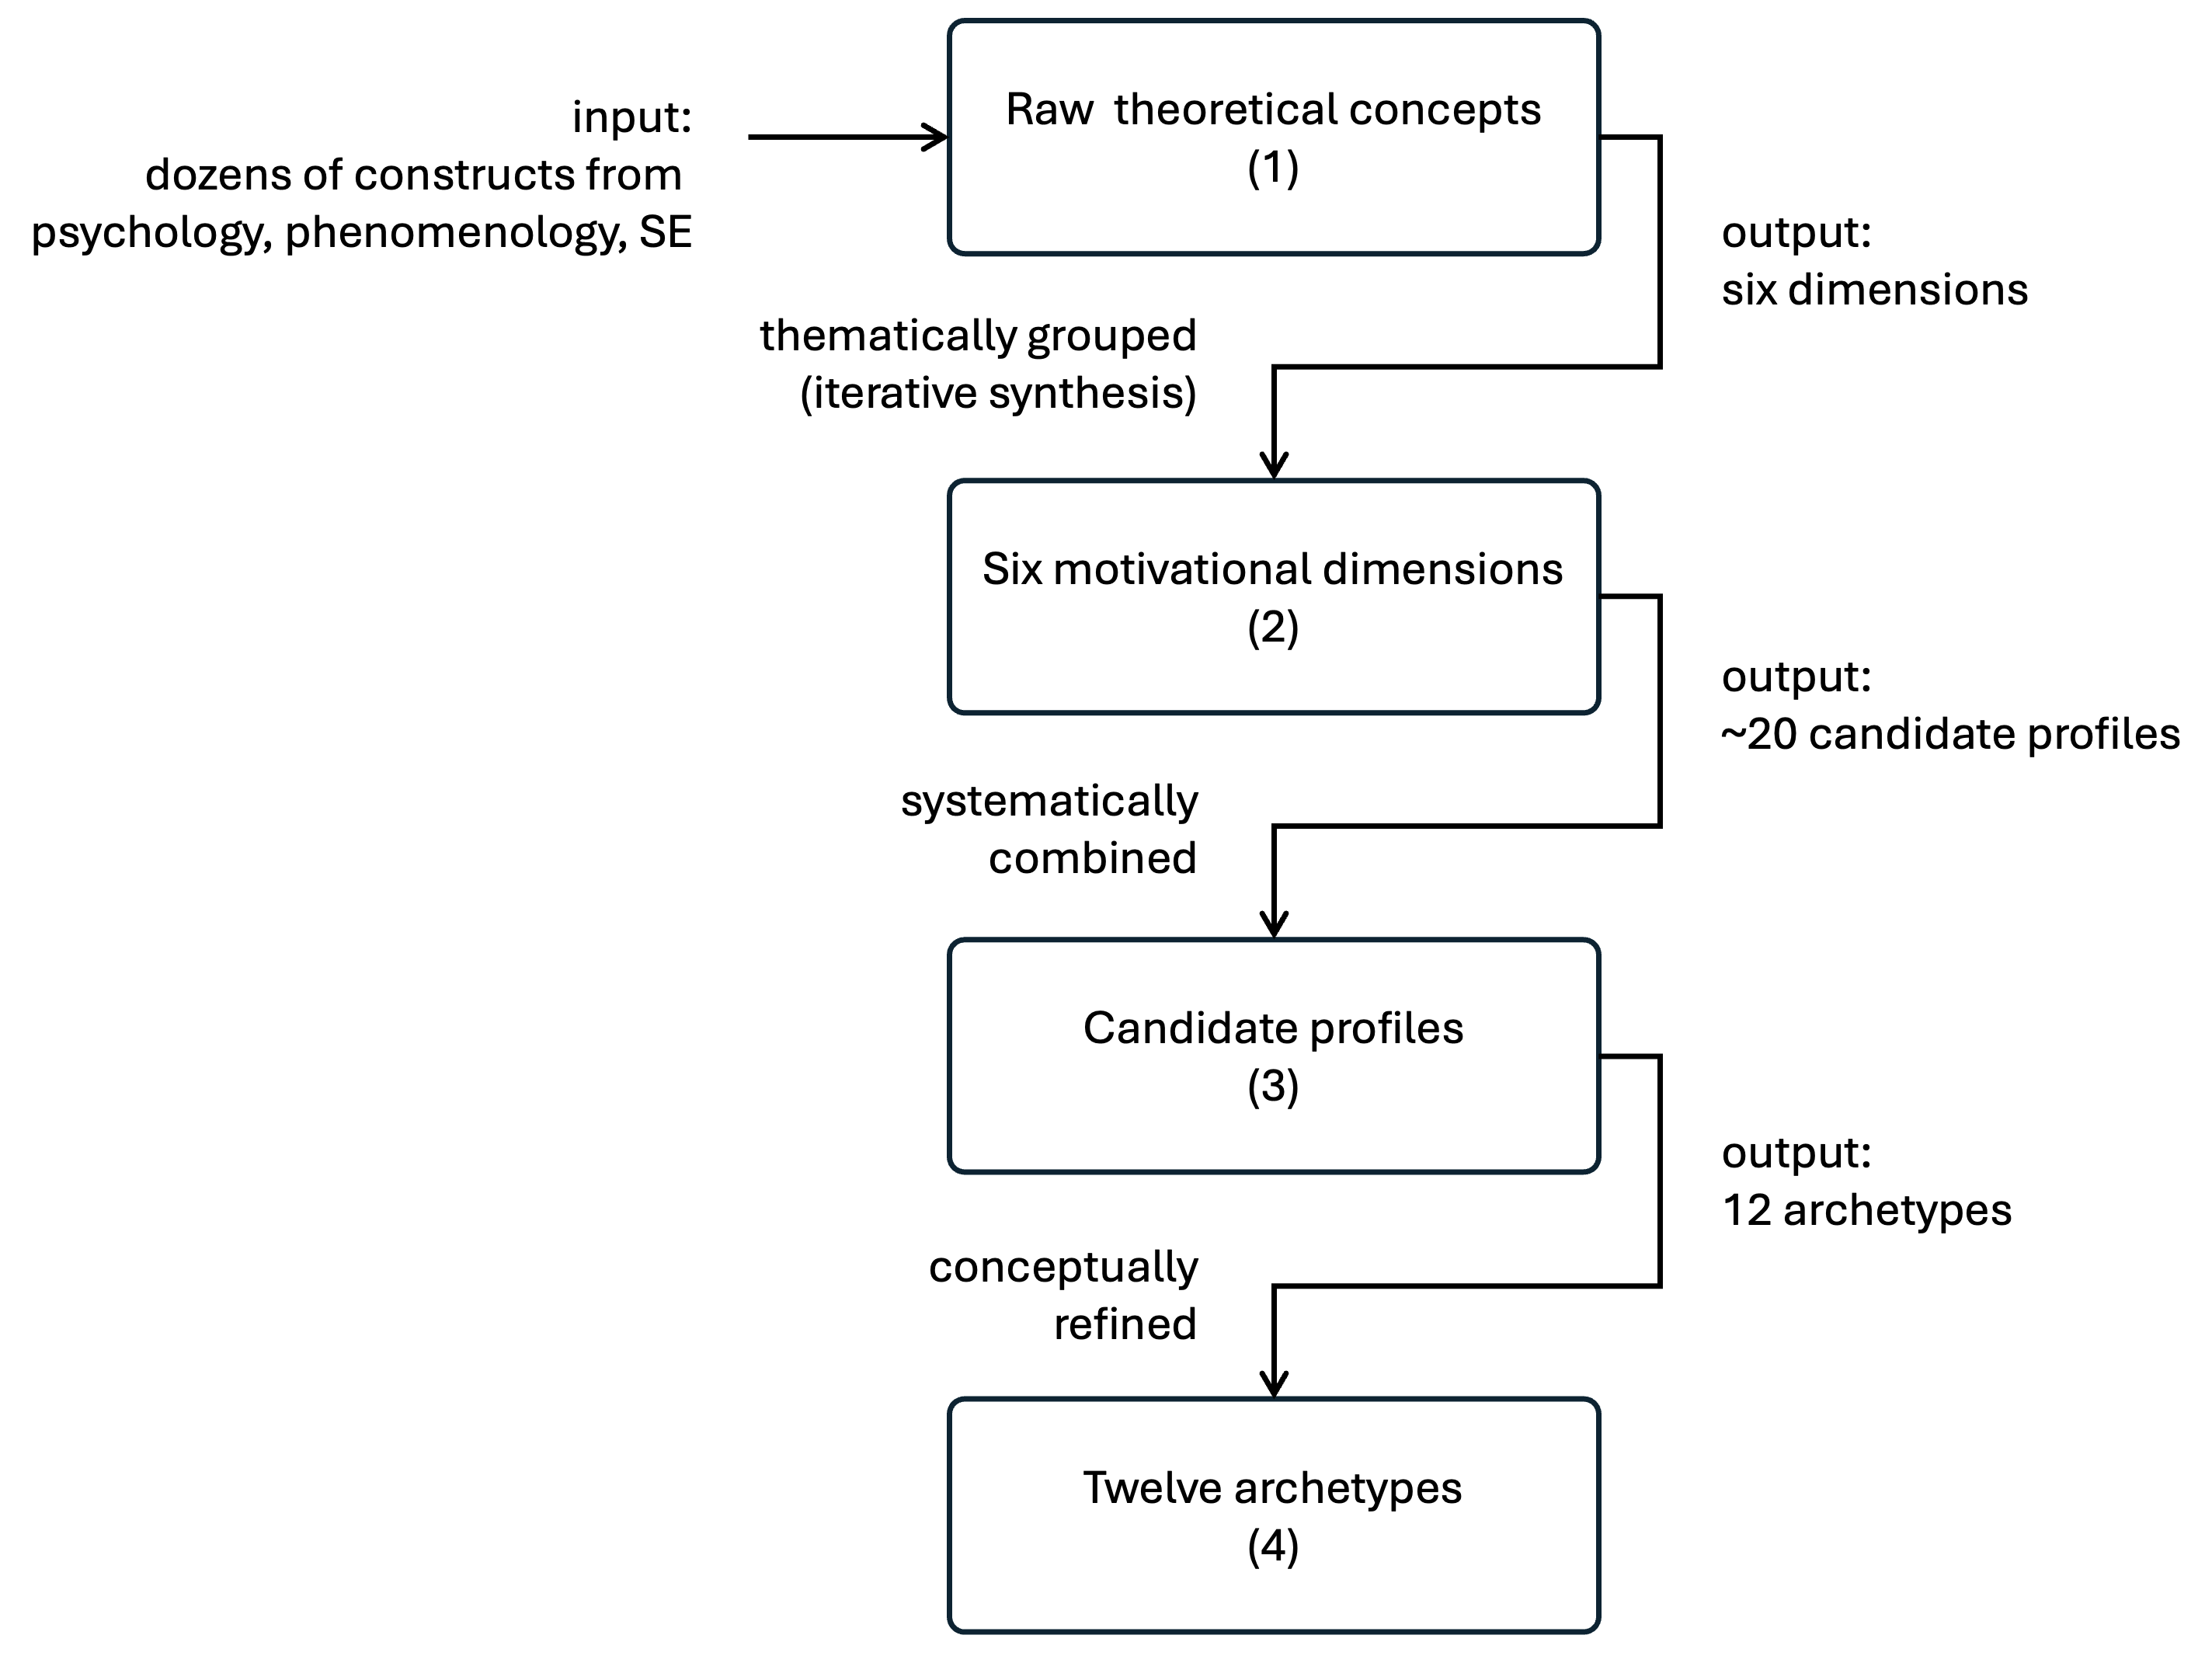
\includegraphics[width=0.5\linewidth]{images/pipeline.png}
    \caption{High-level pipeline for deriving the twelve archetypes. 
    Raw theoretical constructs were synthesized into six motivational 
    dimensions, systematically combined into candidate profiles, and 
    iteratively refined into the final twelve archetypes.}
    \label{fig:pipeline}
\end{figure}

\begin{figure}[htbp]
    \centering
    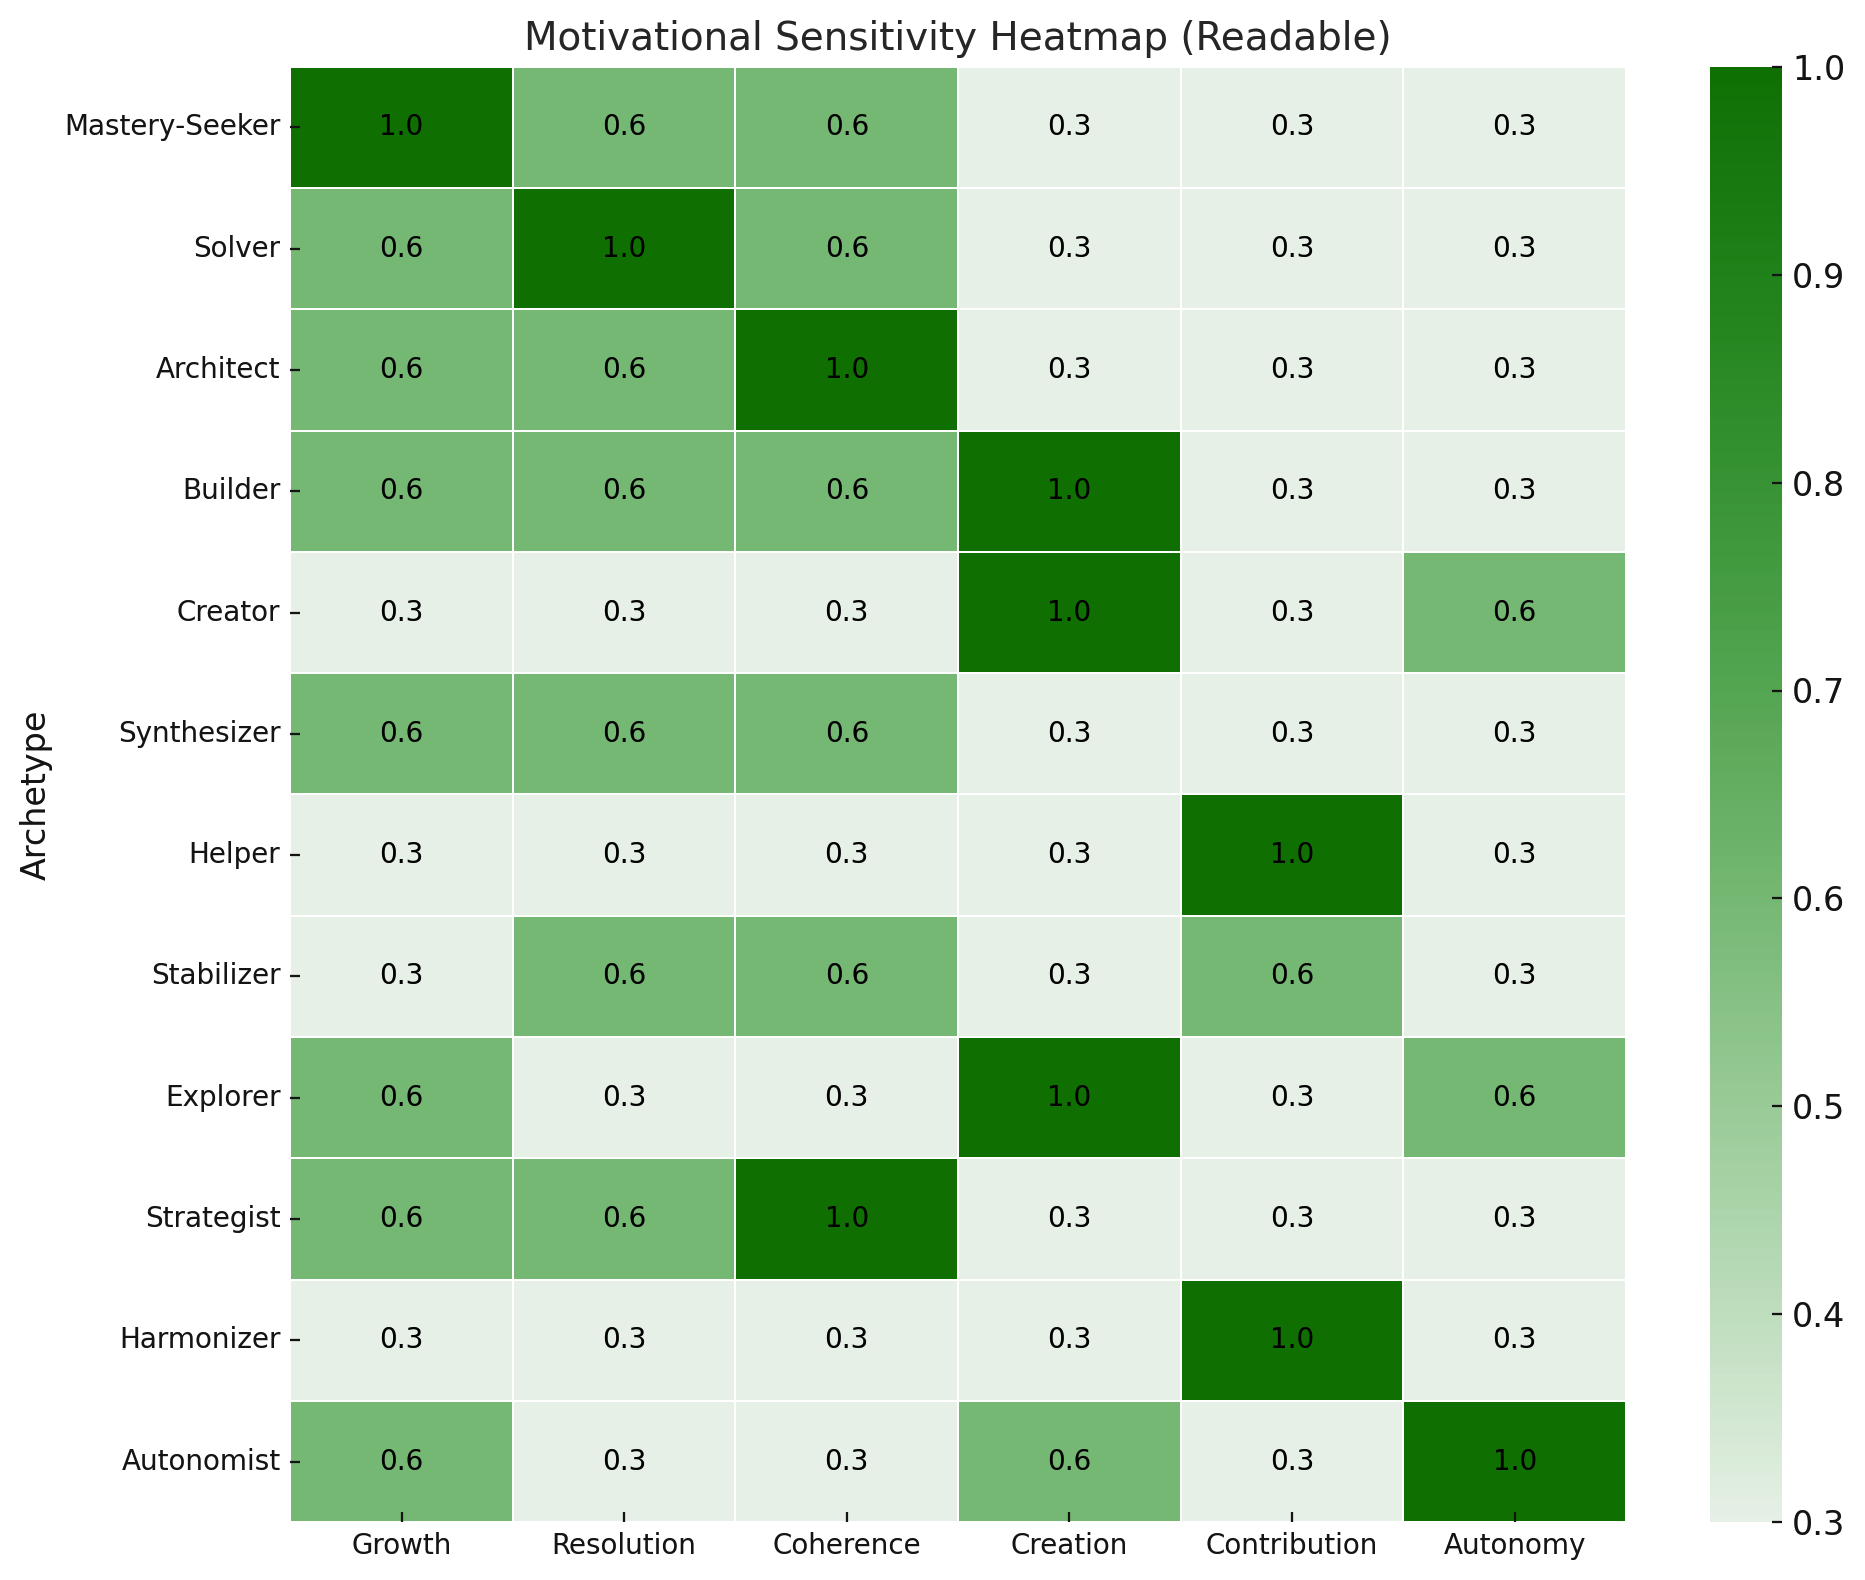
\includegraphics[width=0.7\linewidth]{images/heatmap.png}
    \caption{Heatmap of standardized sensitivity values for the twelve 
    archetypes across the six motivational dimensions. Values follow the 
    ordinal mapping defined in \cref{eq:ordinal}.}
    \label{fig:heatmap}
\end{figure}

% ---------------------------------------------------------------
\section{The Twelve Archetypes of Joy in Software Creation}
\label{sec:archetypes}

The twelve archetypes represent distinct motivational configurations 
through which practitioners experience joy during software creation. 
Each archetype integrates the six motivational dimensions into a stable 
pattern of sensitivity. \Cref{tab:sensitivity} reports the complete 
$12 \times 6$ sensitivity matrix; \cref{fig:radar} illustrates the 
corresponding radar charts.

\begin{table}[htbp]
\caption{Standardized sensitivity values for the twelve archetypes 
across the six motivational dimensions. Dominant\,=\,1.0, 
Secondary\,=\,0.6, Tertiary\,=\,0.3 (see \cref{eq:ordinal}).}
\label{tab:sensitivity}
\centering
\setlength{\tabcolsep}{5pt}
\begin{tabular}{lcccccc}
\toprule
\textbf{Archetype} & \textbf{Gr} & \textbf{Re} & \textbf{Co} 
                   & \textbf{Cr} & \textbf{Cn} & \textbf{Au} \\
\midrule
Mastery-Seeker & 1.0 & 0.6 & 0.3 & 0.0 & 0.0 & 0.0 \\
Solver         & 0.6 & 1.0 & 0.6 & 0.0 & 0.0 & 0.0 \\
Architect      & 0.3 & 0.6 & 1.0 & 0.0 & 0.3 & 0.3 \\
Builder        & 0.6 & 0.6 & 0.3 & 1.0 & 0.0 & 0.0 \\
Creator        & 0.3 & 0.0 & 0.0 & 1.0 & 0.0 & 0.6 \\
Synthesizer    & 0.3 & 0.6 & 1.0 & 0.6 & 0.6 & 0.0 \\
Helper         & 0.3 & 0.6 & 0.0 & 0.0 & 1.0 & 0.3 \\
Stabilizer     & 0.0 & 1.0 & 0.6 & 0.0 & 0.6 & 0.0 \\
Explorer       & 0.6 & 0.0 & 0.0 & 0.6 & 0.3 & 1.0 \\
Strategist     & 0.6 & 0.3 & 0.6 & 0.0 & 1.0 & 0.3 \\
Harmonizer     & 0.3 & 0.6 & 0.6 & 0.0 & 1.0 & 0.3 \\
Autonomist     & 0.0 & 0.3 & 0.0 & 0.3 & 0.3 & 1.0 \\
\bottomrule
\multicolumn{7}{l}{\footnotesize Gr\,=\,Growth, Re\,=\,Resolution, 
Co\,=\,Coherence, Cr\,=\,Creation,}\\
\multicolumn{7}{l}{\footnotesize Cn\,=\,Contribution, Au\,=\,Autonomy.}
\end{tabular}
\end{table}

\begin{figure}[htbp]
    \centering
    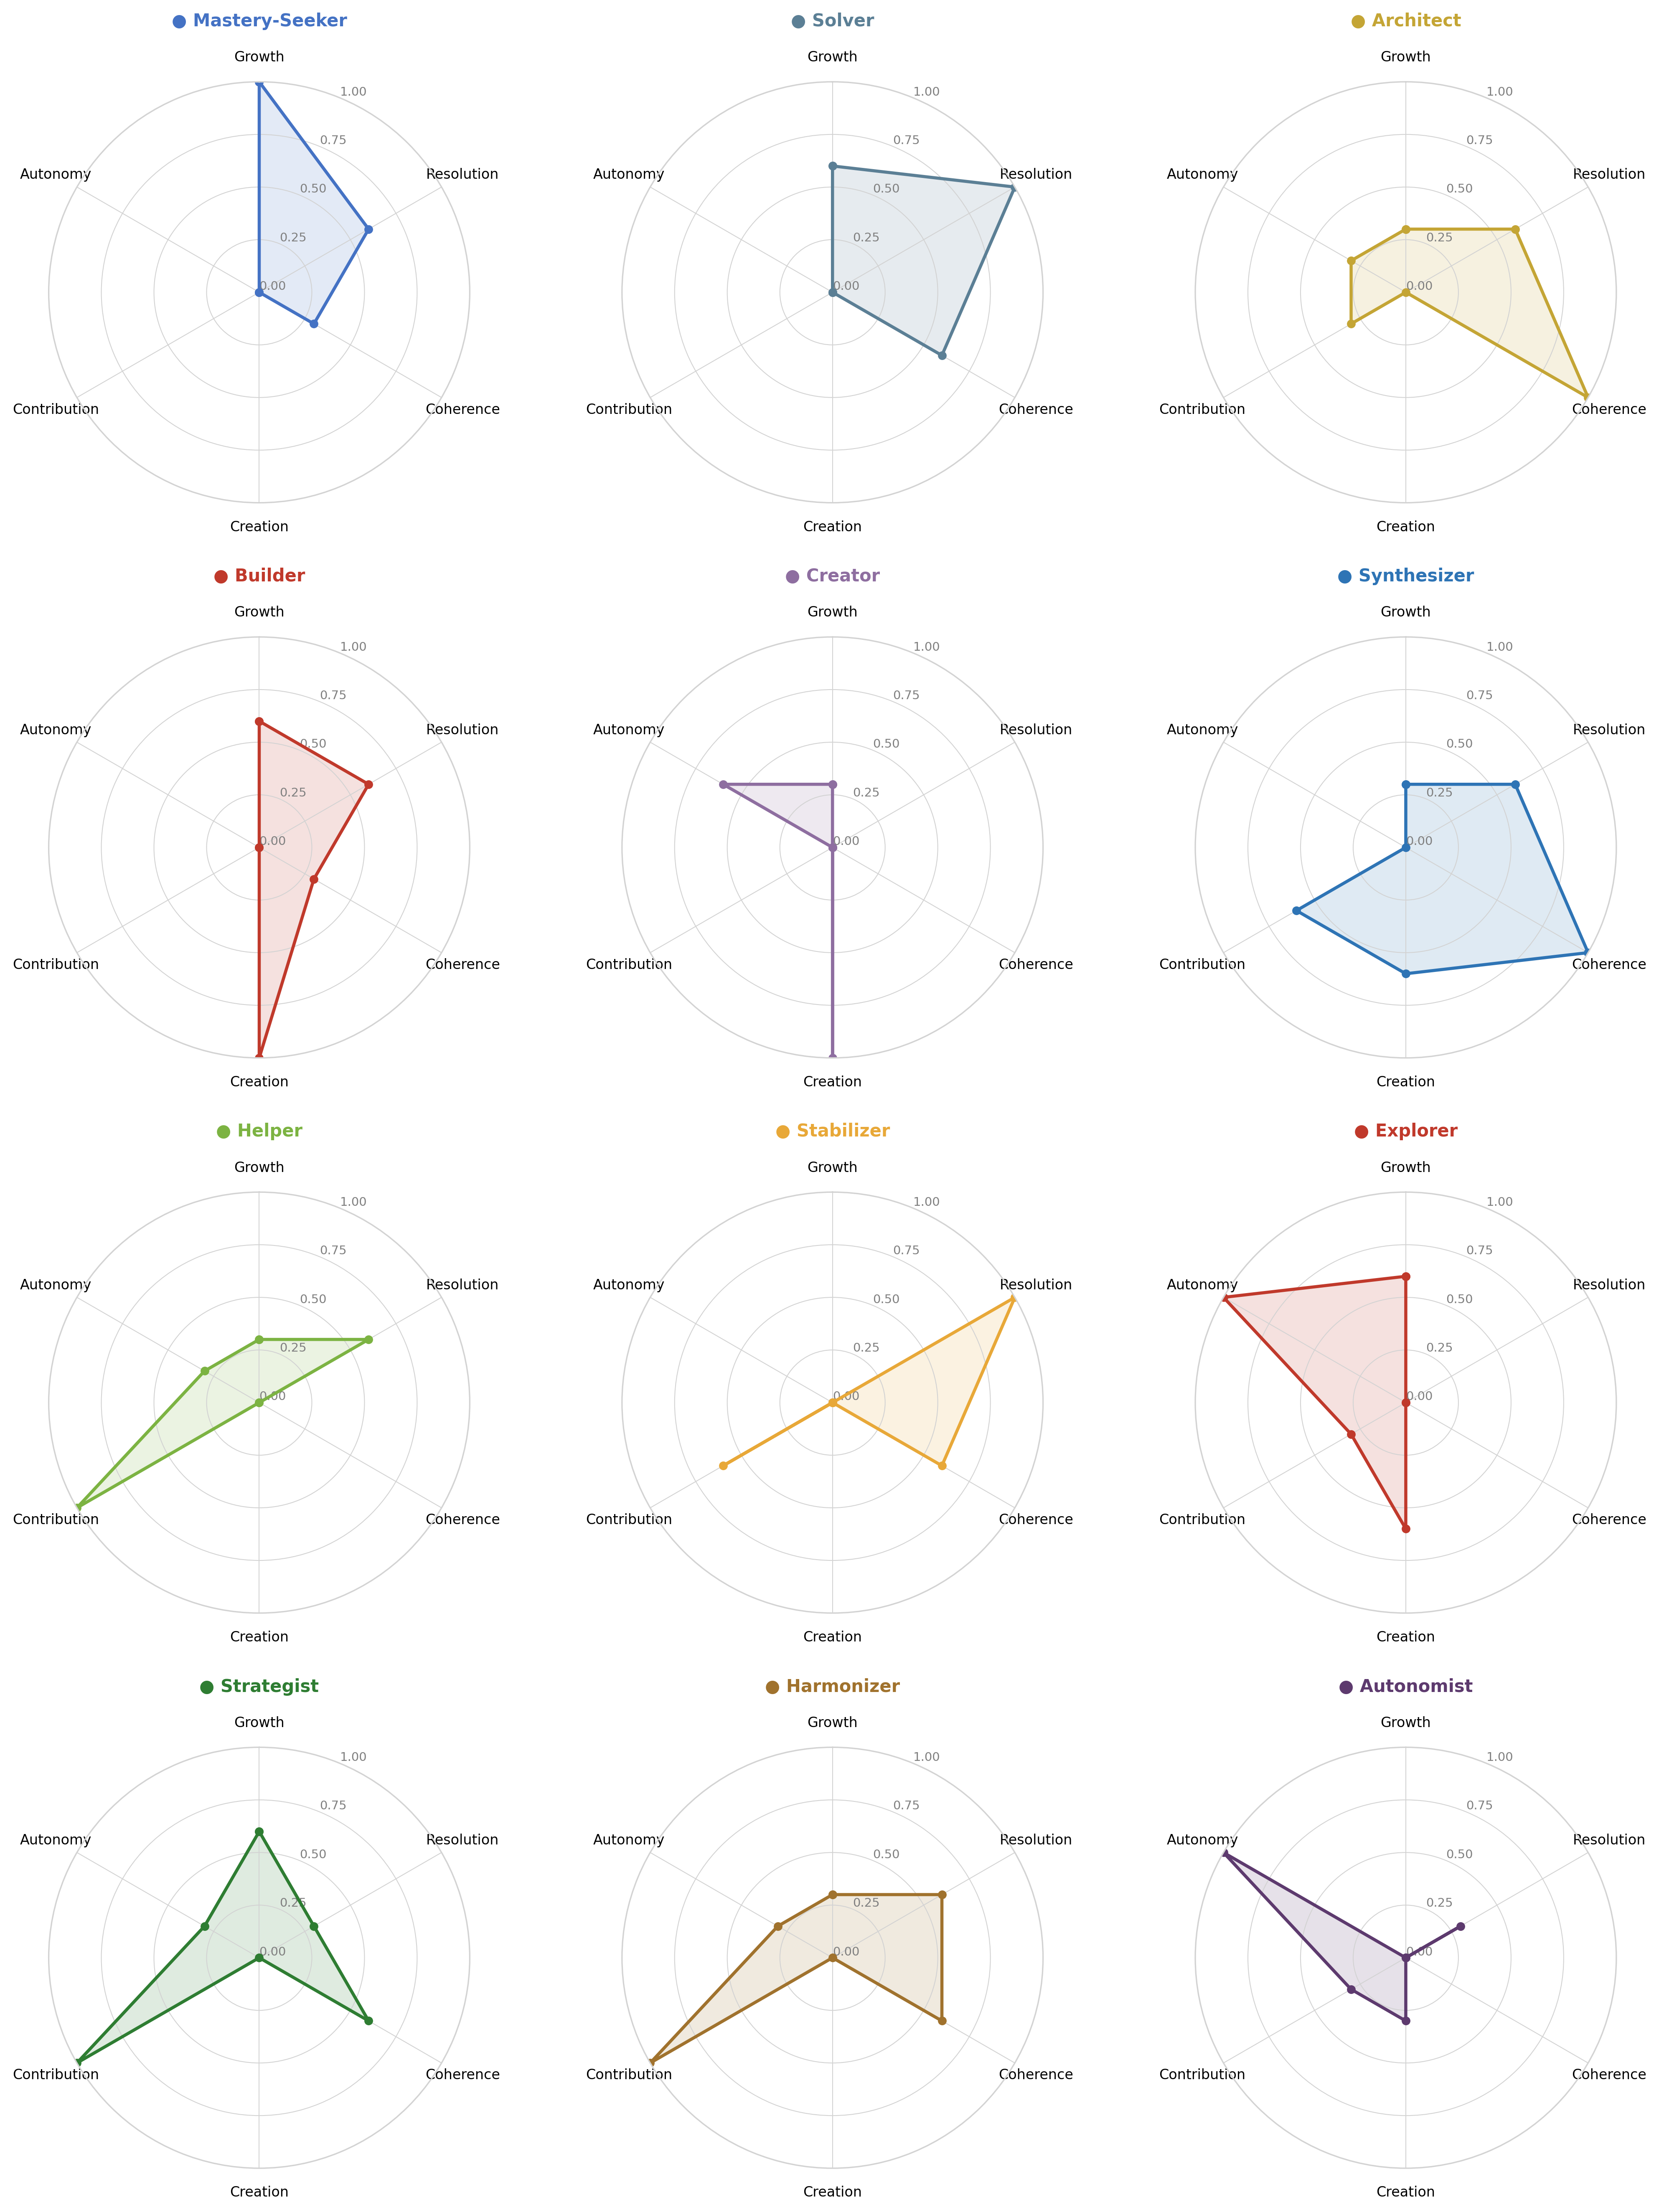
\includegraphics[width=\linewidth]{images/radar.png}
    \caption{Radar charts showing the motivational sensitivity profile 
    of each archetype across the six dimensions. Values are derived 
    using the ordinal mapping scheme in \cref{eq:ordinal}.}
    \label{fig:radar}
\end{figure}

\subsection{Mastery-Seeker}
Mastery-Seekers derive joy primarily from Growth\ldots
% [full archetype descriptions from Sect. VI of original]

% [Repeat \subsection for all 12 archetypes]

% ---------------------------------------------------------------
\section{Modeling the Dynamics of Joy}
\label{sec:model}

\begin{figure}[htbp]
    \centering
    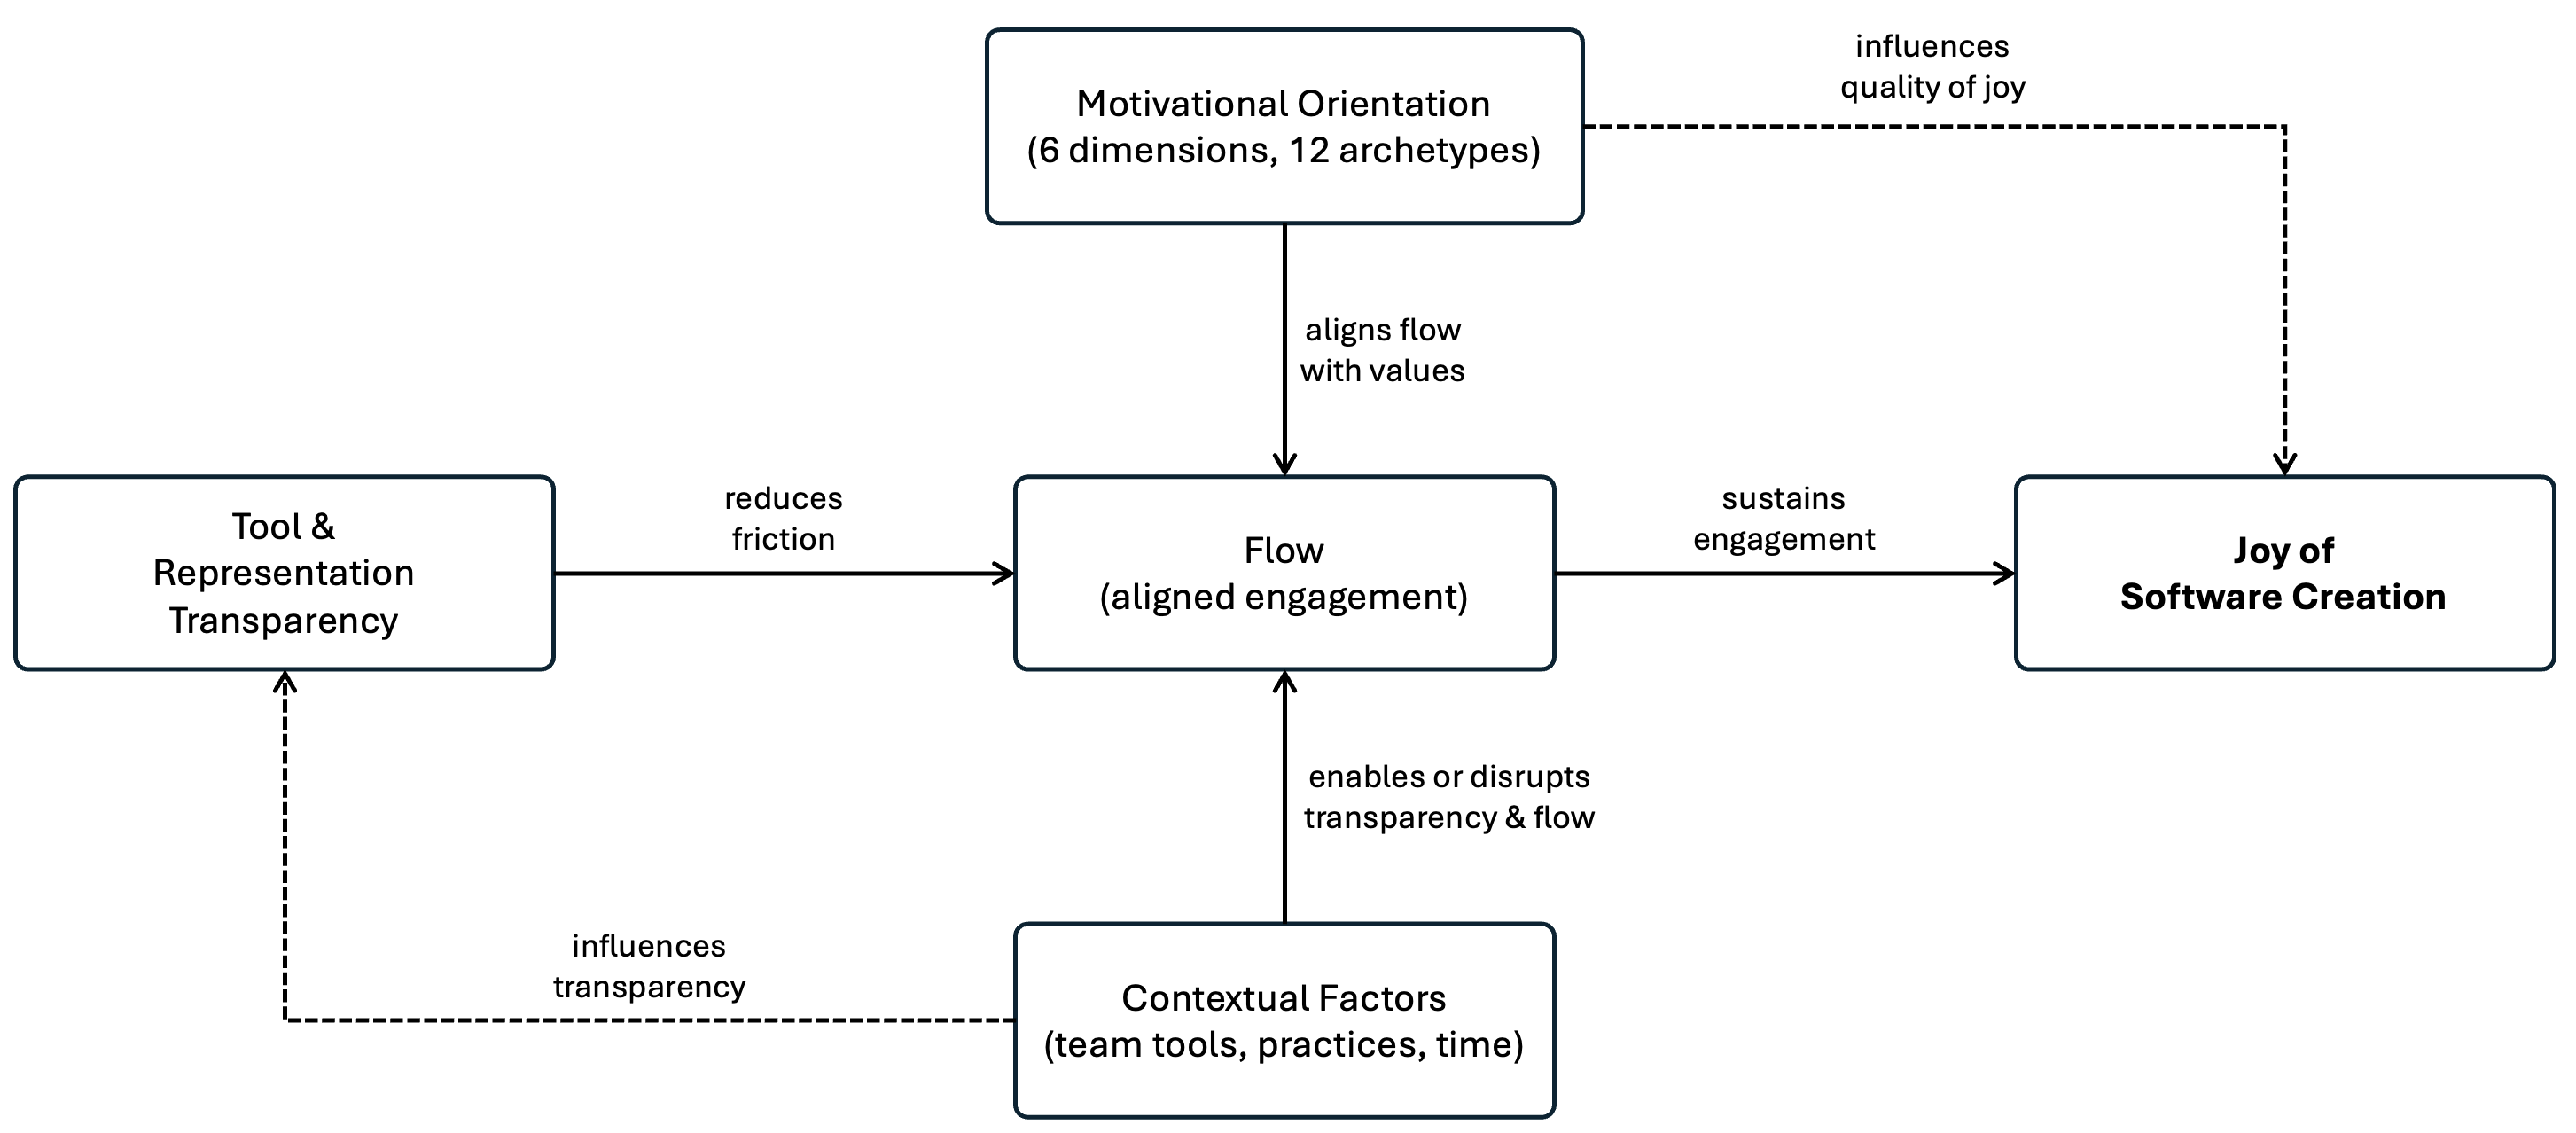
\includegraphics[width=0.85\linewidth]{images/dynamics.png}
    \caption{Conceptual model of the dynamics of joy in software 
    creation. Transparency enables flow by reducing friction; 
    motivational orientation determines whether flow becomes joyful; 
    contextual factors shape the stability and quality of this 
    interaction.}
    \label{fig:model}
\end{figure}

% [Content from Sect. VII of original]

% ---------------------------------------------------------------
\section{Typology Diagram and Cross-Archetype Analysis}
\label{sec:typology}

\begin{figure}[htbp]
    \centering
    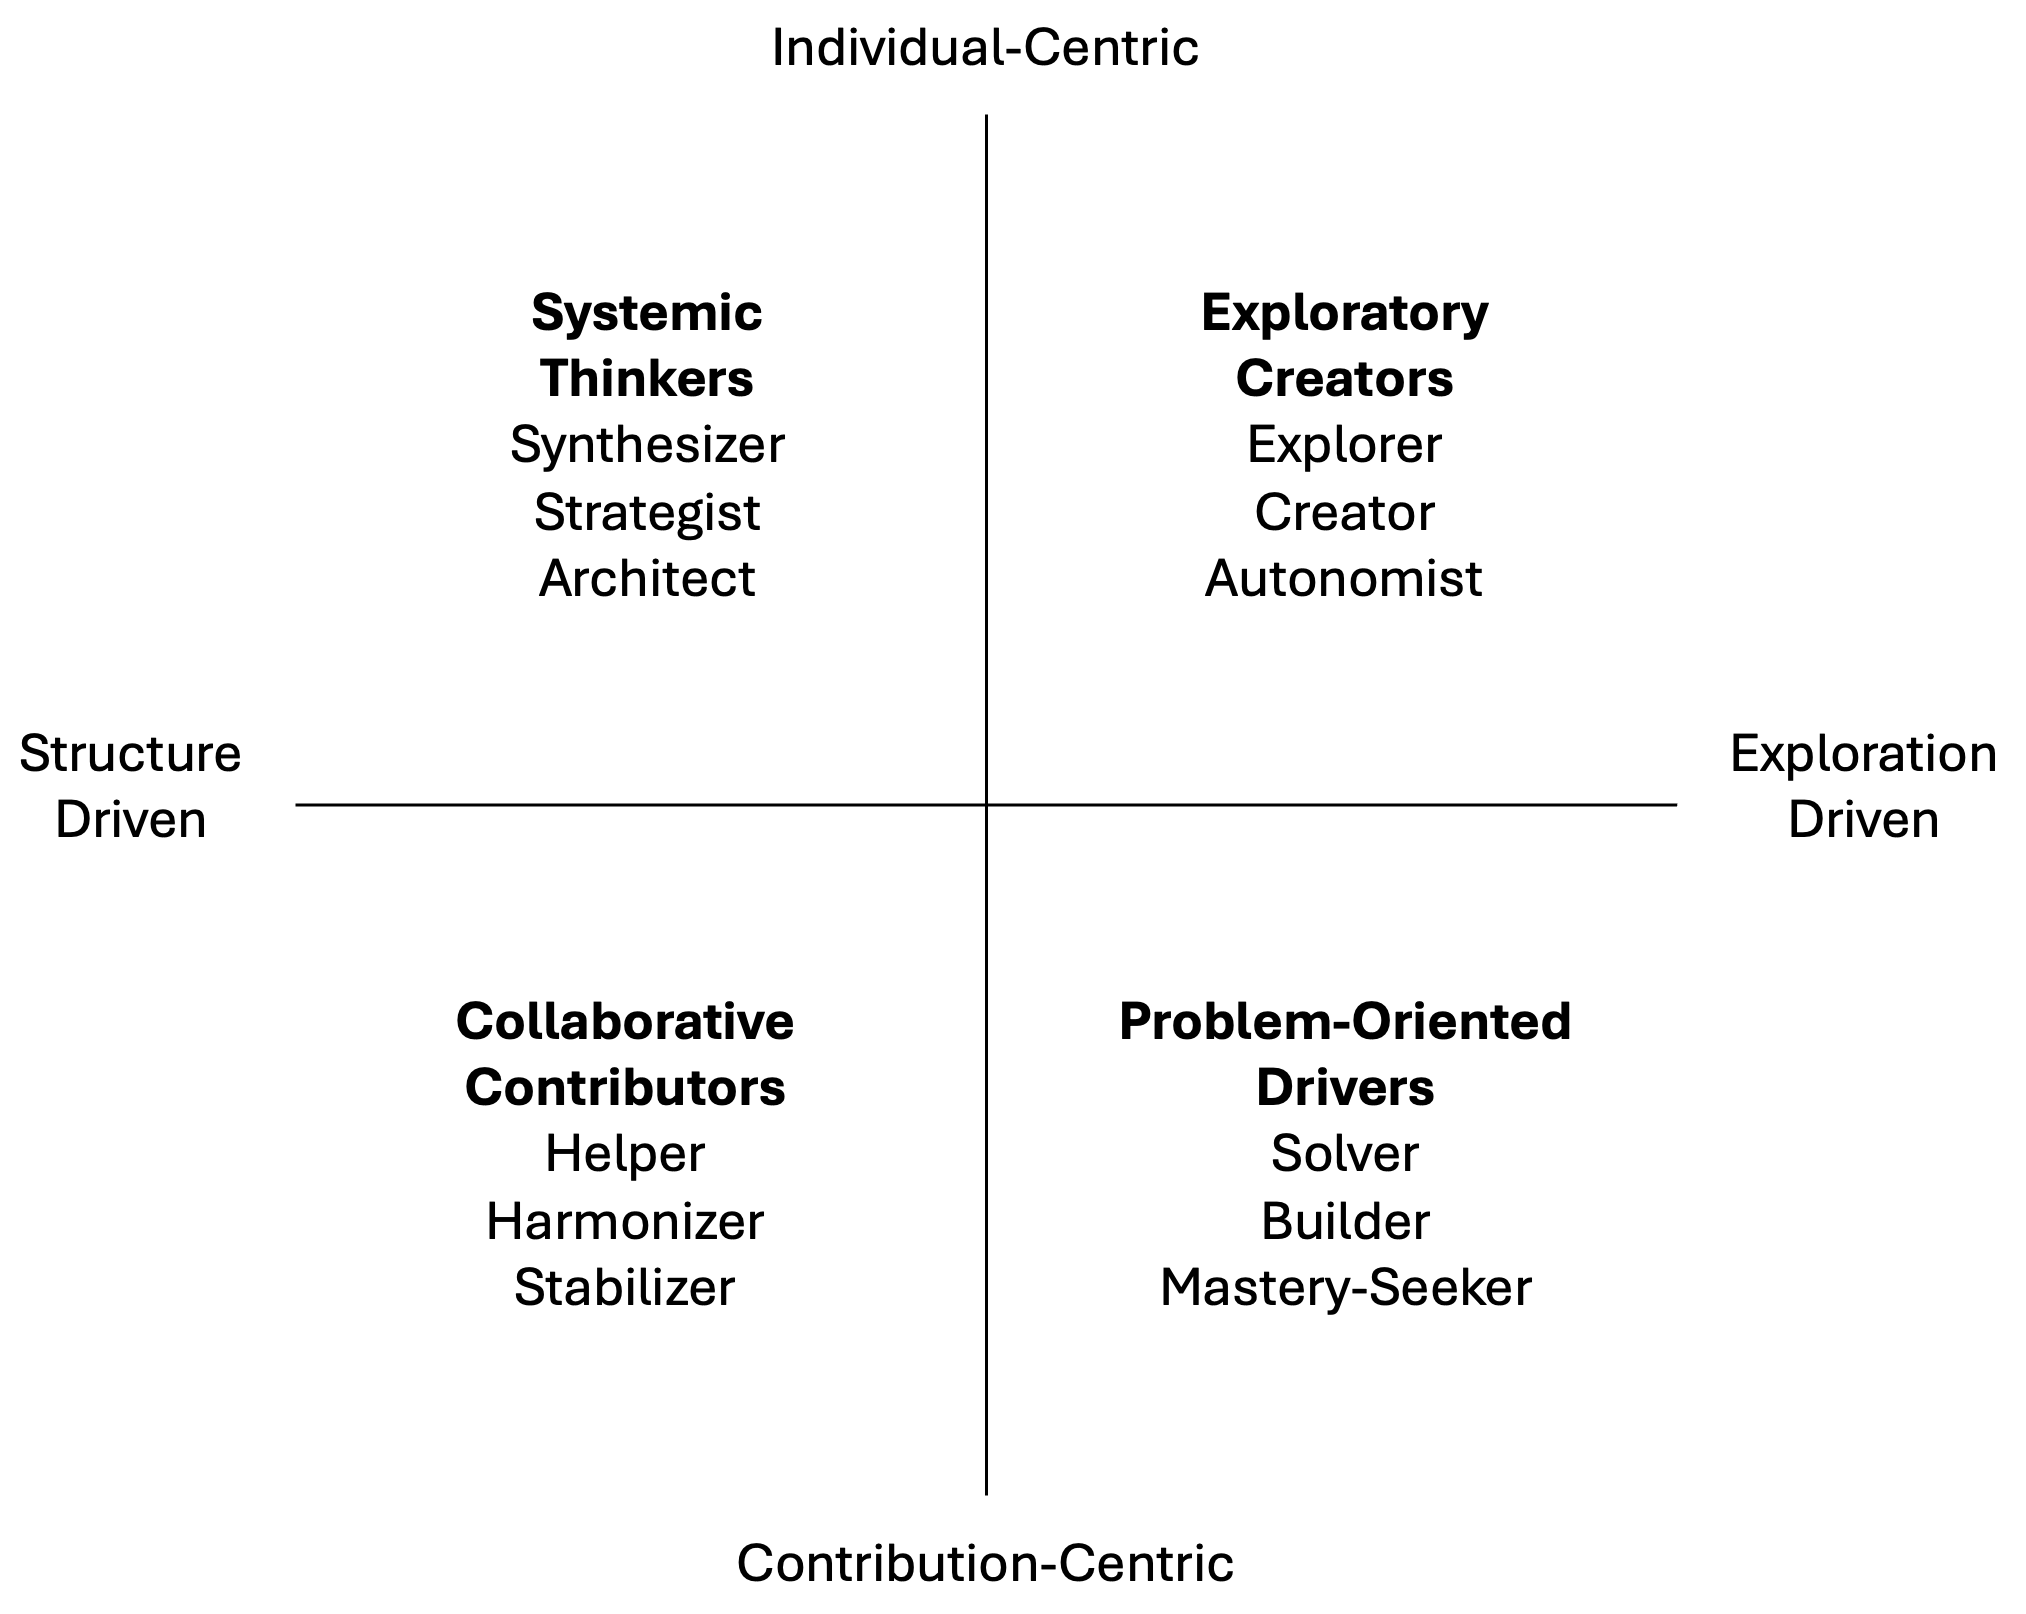
\includegraphics[width=0.6\linewidth]{images/typology-map.png}
    \caption{Conceptual map of the twelve archetypes along two 
    emergent axes: Structure-Driven vs.\ Exploration-Driven 
    motivations (horizontal) and Individual-Centric 
    vs.\ Contribution-Centric orientations (vertical).}
    \label{fig:map}
\end{figure}

% [Content from Sect. VIII of original]

% ---------------------------------------------------------------
\section{Implications for Design}
\label{sec:design}

\begin{table}[htbp]
\caption{Summary of design implications for supporting joy in 
software creation.}
\label{tab:design}
\centering
\begin{tabularx}{\linewidth}{lX}
\toprule
\textbf{Design Focus} & \textbf{Key Implications} \\
\midrule
Transparency \& Friction Reduction &
    Minimize cognitive and phenomenological friction; reduce 
    context-switching; simplify visual and textual noise; stabilize 
    feedback loops; ensure predictable interactions; support continuity 
    of thought; provide representations aligned with the cognitive grain 
    of the task. \\
\addlinespace
Motivational Diversity &
    Support configurable workflows (structured vs.\ free-form); offer 
    multiple representational views; adaptively surface features suited 
    to motivational profiles; enhance opportunities for contribution; 
    preserve autonomy through customization and local control. \\
\addlinespace
Socio-Technical Environment &
    Balance challenge and skill; respect attentional rhythms; provide 
    role flexibility; create teams with complementary archetypes; adapt 
    workflows and practices rather than individuals to accommodate 
    cognitive diversity. \\
\addlinespace
Holistic Alignment &
    Recognize that joy emerges only when motivational needs, tool 
    affordances, and organizational conditions are aligned; design for 
    continuity, autonomy, contribution, or exploration according to the 
    archetype. \\
\bottomrule
\end{tabularx}
\end{table}

% [Detailed content from Sect. IX of original]

% ---------------------------------------------------------------
\section{Threats to Validity}
\label{sec:threats}

% [Content from Threats section of original, expanded per review
%  suggestions: inter-rater, confirmation bias, empirical validation]

% ---------------------------------------------------------------
\section{Conclusion}
\label{sec:conclusion}

% [Content from Sect. X of original]

% ---------------------------------------------------------------
%% ACKNOWLEDGEMENTS
%% ---------------------------------------------------------------
\section*{Acknowledgements}

The research presented in this paper is partially funded by the 
European Union under the Grant Agreement No.\ 101189664. Views and 
opinions expressed are however those of the authors only and do not 
necessarily reflect those of the European Union or the European Health 
and Digital Executive Agency (HADEA). Neither the European Union nor 
the granting authority can be held responsible for them.

% ---------------------------------------------------------------
%% CRediT AUTHOR CONTRIBUTION STATEMENT (Elsevier requirement)
%% ---------------------------------------------------------------
\section*{CRediT authorship contribution statement}

\textbf{Alfonso Pierantonio:} Conceptualization, Methodology, 
Writing -- original draft, Writing -- review \& editing, 
Supervision, Funding acquisition.
\textbf{Bernhard Schenkenfelder:} Conceptualization, 
Writing -- original draft, Writing -- review \& editing.

% ---------------------------------------------------------------
%% DECLARATION OF COMPETING INTERESTS
%% ---------------------------------------------------------------
\section*{Declaration of competing interests}

The authors declare that they have no known competing financial 
interests or personal relationships that could have appeared to 
influence the work reported in this paper.

% ---------------------------------------------------------------
%% DATA AVAILABILITY
%% ---------------------------------------------------------------
\section*{Data availability}

No data was used for the research described in this article.

% ---------------------------------------------------------------
%% BIBLIOGRAPHY
%% ---------------------------------------------------------------
\bibliography{references}

%% ---------------------------------------------------------------
%% APPENDIX (optional — raw constructs table can go here)
%% ---------------------------------------------------------------
\appendix

\section{Raw Theoretical Constructs}
\label{app:constructs}

\begin{table}[htbp]
\caption{Raw theoretical constructs used as inputs to the motivational 
synthesis.}
\label{tab:constructs}
\centering
\begin{tabularx}{\linewidth}{lXl}
\toprule
\textbf{Source Domain} & \textbf{Example Constructs} & \textbf{Refs} \\
\midrule
Motivation Psychology & 
    Intrinsic motivation; mastery orientation; autonomy; competence; 
    relatedness; goal-directed behavior; challenge--skill balance & 
    \cite{ryan2000,csikszentmihalyi1990} \\
\addlinespace
Reward Sensitivity & 
    Reward responsiveness; approach--avoidance tendencies; 
    sensitivity to feedback; reinforcement history & 
    \cite{gray1987,corr2004} \\
\addlinespace
Cognitive Styles & 
    Systemizing; holistic vs.\ analytic reasoning; coherence seeking; 
    abstraction preference; exploratory vs.\ structured 
    problem-solving & 
    \cite{messick1976,kirton1984} \\
\addlinespace
Flow Theory & 
    Attentional absorption; loss of self-consciousness; cognitive 
    momentum; immediacy of feedback; sense of control & 
    \cite{csikszentmihalyi1990,nakamura2009} \\
\addlinespace
Phenomenology & 
    Tool transparency; readiness-to-hand; embodied interaction; 
    mediation; technological appropriation & 
    \cite{heidegger1962,ihde1990} \\
\addlinespace
SE Cognition \& DX & 
    Cognitive load; problem-solving strategies; abstraction use; 
    task interruptions; representational alignment; tooling friction & 
    \cite{green1996,parnin2011,kramer2007} \\
\bottomrule
\end{tabularx}
\end{table}

\end{document}
